%%%%%%%%%%%%%%%%%%%%%%%%%%%%%%%%%%%%%%%%%
% Short Sectioned Assignment LaTeX Template Version 1.0 (5/5/12)
% This template has been downloaded from: http://www.LaTeXTemplates.com
% Original author:  Frits Wenneker (http://www.howtotex.com)
% License: CC BY-NC-SA 3.0 (http://creativecommons.org/licenses/by-nc-sa/3.0/)
%%%%%%%%%%%%%%%%%%%%%%%%%%%%%%%%%%%%%%%%%

%----------------------------------------------------------------------------------------
%	PACKAGES AND OTHER DOCUMENT CONFIGURATIONS
%----------------------------------------------------------------------------------------

\documentclass[paper=a4, fontsize=11pt]{scrartcl} % A4 paper and 11pt font size

% ---- Entrada y salida de texto -----

\usepackage[T1]{fontenc} % Use 8-bit encoding that has 256 glyphs
\usepackage[utf8]{inputenc}
%\usepackage{fourier} % Use the Adobe Utopia font for the document - comment this line to return to the LaTeX default

% ---- Idioma --------
\usepackage[spanish]{babel}
%\usepackage[spanish]{babel} % Selecciona el español para palabras introducidas automáticamente, p.ej. "septiembre" en la fecha y especifica que se use la palabra Tabla en vez de Cuadro

% ---- Otros paquetes ----

\usepackage{url} % ,href} %para incluir URLs e hipervínculos dentro del texto (aunque hay que instalar href)
\usepackage{amsmath,amsfonts,amsthm} % Math packages
%\usepackage{graphics,graphicx, floatrow} %para incluir imágenes y notas en las imágenes
\usepackage{graphics,graphicx, float} %para incluir imágenes y colocarlas

% Para hacer tablas comlejas
%\usepackage{multirow}
%\usepackage{threeparttable}

%\usepackage{sectsty} % Allows customizing section commands
%\allsectionsfont{\centering \normalfont\scshape} % Make all sections centered, the default font and small caps

\usepackage{fancyhdr} % Custom headers and footers
\pagestyle{fancyplain} % Makes all pages in the document conform to the custom headers and footers
\fancyhead{} % No page header - if you want one, create it in the same way as the footers below
\fancyfoot[L]{} % Empty left footer
\fancyfoot[C]{} % Empty center footer
\fancyfoot[R]{\thepage} % Page numbering for right footer
\renewcommand{\headrulewidth}{0pt} % Remove header underlines
\renewcommand{\footrulewidth}{0pt} % Remove footer underlines
\setlength{\headheight}{13.6pt} % Customize the height of the header

\numberwithin{equation}{section} % Number equations within sections (i.e. 1.1, 1.2, 2.1, 2.2 instead of 1, 2, 3, 4)
\numberwithin{figure}{section} % Number figures within sections (i.e. 1.1, 1.2, 2.1, 2.2 instead of 1, 2, 3, 4)
\numberwithin{table}{section} % Number tables within sections (i.e. 1.1, 1.2, 2.1, 2.2 instead of 1, 2, 3, 4)

\setlength\parindent{0pt} % Removes all indentation from paragraphs - comment this line for an assignment with lots of text

\newcommand{\horrule}[1]{\rule{\linewidth}{#1}} % Create horizontal rule command with 1 argument of height

\graphicspath{ {./images/} }
\usepackage{subcaption}
\usepackage{hyperref}
\usepackage{soul}


%----------------------------------------------------------------------------------------
%	TÍTULO Y DATOS DEL ALUMNO
%----------------------------------------------------------------------------------------

\title{	
\normalfont \normalsize 
\textsc{\textbf{Series Temporales y Minería de Flujo de Datos (2019-2020)} \\ Máster Oficial Universitario en Ciencia de Datos e Ingeniería de Computadores \\ Universidad de Granada} \\ [25pt] % Your university, school and/or department name(s)
\horrule{0.5pt} \\[0.4cm] % Thin top horizontal rule
\huge Trabajo autónomo I: Series Temporales \\ % The assignment title
\horrule{2pt} \\[0.5cm] % Thick bottom horizontal rule
}

\author{Luis Balderas Ruiz \\ \texttt{luisbalderas@correo.ugr.es}} 
 % Nombre y apellidos 


\date{\normalsize\today} % Incluye la fecha actual

%----------------------------------------------------------------------------------------
% DOCUMENTO
%----------------------------------------------------------------------------------------

\begin{document}

\maketitle % Muestra el Título

\newpage %inserta un salto de página

\tableofcontents % para generar el índice de contenidos

\listoffigures

\listoftables

\newpage

%
%\begin{figure}[H] %con el [H] le obligamos a situar aquí la figura
%	\centering
%	\includegraphics[scale=0.6]{e1.png}  %el parámetro scale permite agrandar o achicar la imagen. En el nombre de archivo puede especificar directorios
%	\caption{Progresión de la imagen de E en cada iteración} 
%	\label{fig:e1}
%\end{figure}

\section{PARTE TEÓRICA}

\subsection{Introducción}

En la presente sección se justifican, desde un punto de vista teórico, las distintas decisiones tomadas para estudiar la Estación 2870, correspondiente a Salamanca, para acabar haciendo predicciones a nivel diario (los siete primeros días de marzo de 2018) y mensual (marzo y abril de 2018) sobre la temperatura máxima registrada en dicha estación. 

\subsection{Preprocesamiento}

El preprocesamiento es una de las partes más importantes en el proceso de adquisición de conocimiento. Bien conocidas son las gráficas que indican que la mayoría del tiempo invertido por los científicos de datos se emplea en limpiar y preparar los datos (\cite{prep-time}), así como proverbios como 'Garbage in, garbage out' (\cite{gigo}). En series temporales, esto no es una excepción. Tras la lectura de datos de la estación, que recogen diversas medidas atmosféricas diariamente, y la creación de nuevas características como Día y Mes, para así poder agrupar las instancias más cómodamente, estudio la correlación de las variables numéricas, que estudian las temperaturas máximas, mínimas y medias de cada día junto con velocidades de viento y nivel de precipitaciones:

\begin{figure}[H] %con el [H] le obligamos a situar aquí la figura
	\centering
	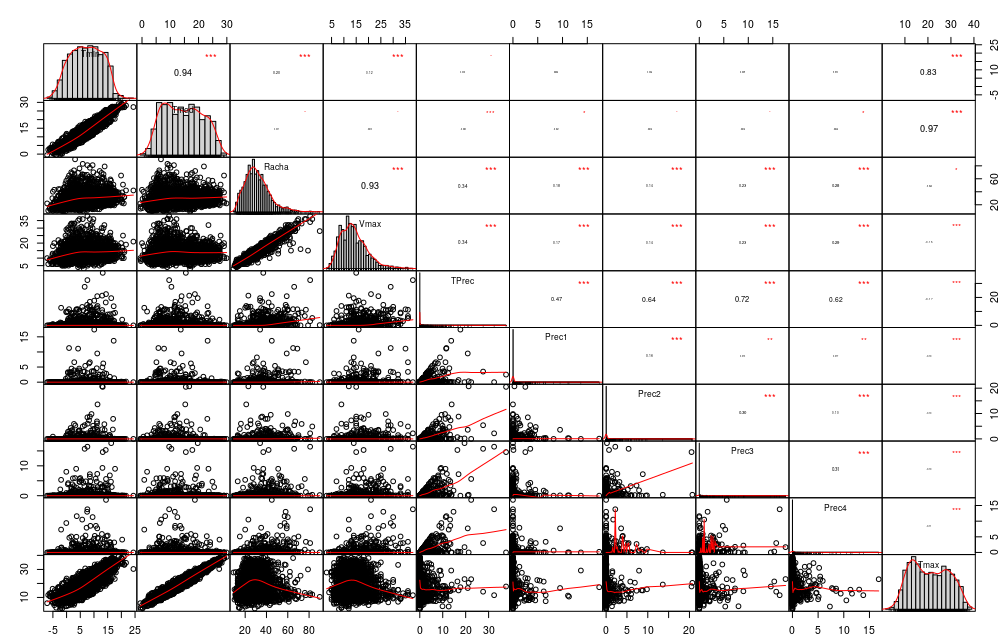
\includegraphics[scale=0.4]{correlation.png}  %el parámetro scale permite agrandar o achicar la imagen. En el nombre de archivo puede especificar directorios
	\caption{Correlación de las variables con el target Temperatura máxima} 
	\label{fig:corr}
\end{figure}

Teniendo en cuenta que nuestro objetivo es modelar la temperatura máxima, la enfrentamos con el resto de variables, de manera que vemos que existe una alta correlación entre la temperatura máxima y la media (97\%) y la máxima y la mínima (83\%). Esto nos podría ser de ayuda para posteriores imputaciones de valores perdidos (que será la parte fundamental del preprocesamiento, debido a la alta cantidad de ellos). A continuación, estudio si existen anomalías en la temperatura máxima (vía el rango intercuartílico) con resultado negativo. Por tanto, me centro en la imputación de valores perdidos. En \cite{na1} encontramos distintos enfoques para tratar con \textit{missing values} en series temporales, desde ignorarlos, borrarlos, imputaciones con estadísticos como la media, mediana, moda; y otro más elaborados por medio de modelos autoregresivos, basados en algoritmos genéticos, interpolación, medidas de similaridad o clasificadores como SVM o kNN. Utilizo el paquete de R \textit{imputeTS} (\cite{RJ-2017-009}), especializado en imputación de series temporales univariables. En primer lugar, estudiamos la distribución de valores perdidos y la situamos temporalmente:

\begin{figure}[H] %con el [H] le obligamos a situar aquí la figura
	\centering
	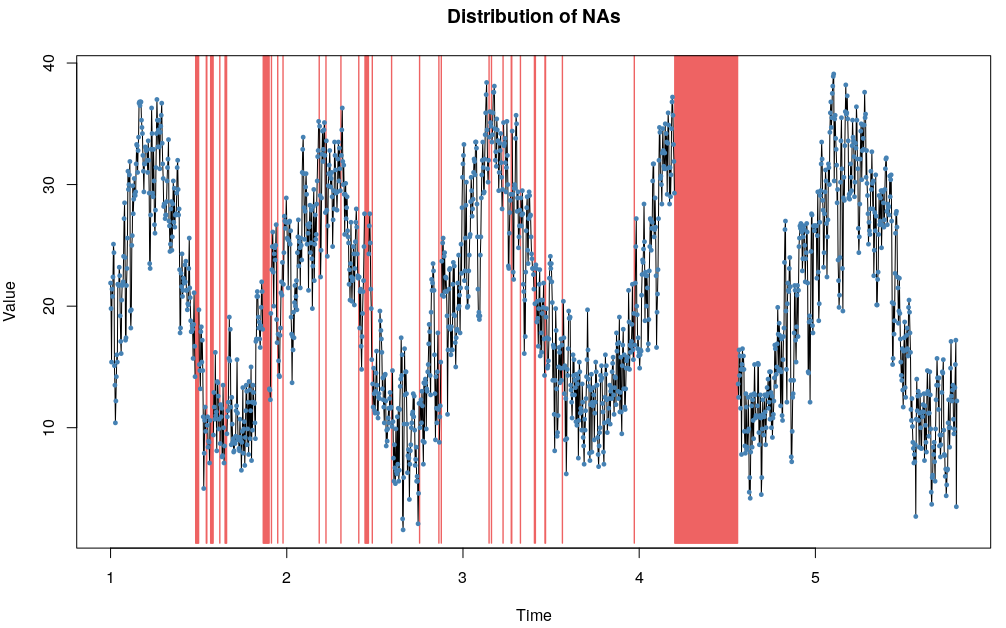
\includegraphics[scale=0.42]{na-dist.png}  %el parámetro scale permite agrandar o achicar la imagen. En el nombre de archivo puede especificar directorios
	\caption{Distribución de valores perdidos en la serie temporal} 
	\label{fig:na-dist}
\end{figure}

viendo que una gran parte de datos perdidos se encuentra entre el periodo 4 y 5, es decir, en el año 2017. Más concretamente, vemos que en la franja temporal de entre el 67\% y el 75\% de tiempo se encuentra el 80\% de los valores perdidos.

\begin{figure}[H] %con el [H] le obligamos a situar aquí la figura
	\centering
	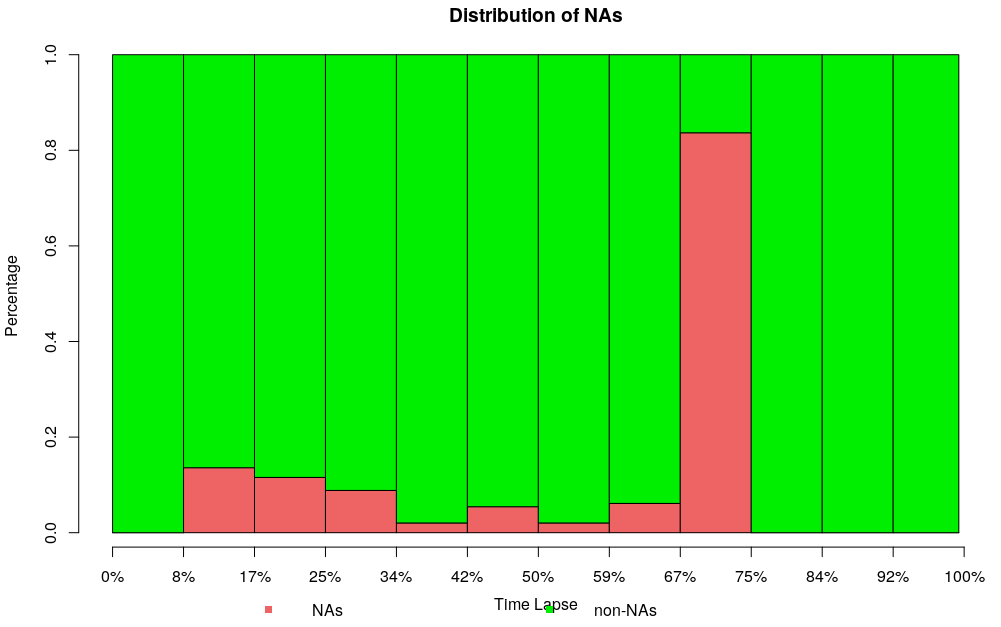
\includegraphics[scale=0.23]{nadistbar.png}  %el parámetro scale permite agrandar o achicar la imagen. En el nombre de archivo puede especificar directorios
	\caption{Distribución de valores perdidos en la serie temporal con lapso de tiempo} 
	\label{fig:na-distbar}
\end{figure}

Además, tras una exploración de datos, vemos que todas las mediciones de esos días están perdidas, probablemente por un avería del dispositivo. Esto nos hace descartar la posibilidad de imputar valores vía a las variables más correladas a la temperatura máxima. Tras el estudio de ciertas estadísticas más, pruebo varias funciones de imputación del paquete. Entre ellas, LOFC (imputación por la última observación considerada), NOFC, medias móviles, la imputación de modelo estructural y suavizado de Kalman,  Seadec (imputación basada en la descomposición de la estacionalidad) y Seasplit (imputación basada en la partición de la estacionalidad). Acabo adoptando esta última, porque visualmente parece la más acertada, ya que las otras imputan los valores de una forma muy lineal, lo que difiere del comportamiento normal de la serie, con cierta fluctuación y diente de sierra.

\begin{figure}[H] %con el [H] le obligamos a situar aquí la figura
	\centering
	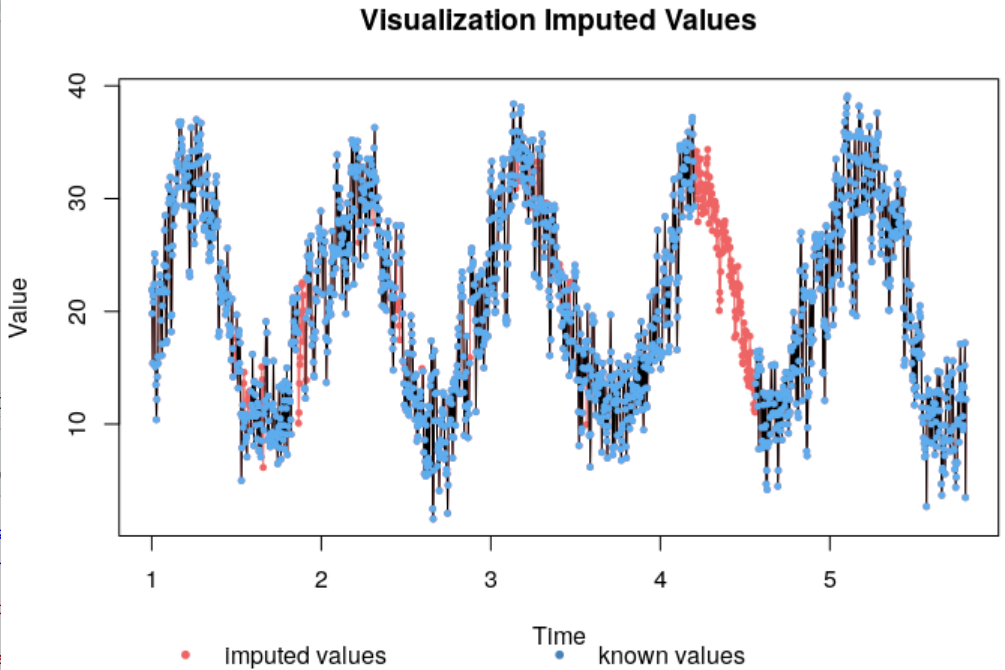
\includegraphics[scale=0.24]{seasplit-na.png}  %el parámetro scale permite agrandar o achicar la imagen. En el nombre de archivo puede especificar directorios
	\caption{Resultado de la imputación de valores perdidos con Seasplit} 
	\label{fig:seasplit}
\end{figure}

Tras imputar los valores perdidos, es momento de generar las series, diaria y mensual, que me servirá para modelar y predecir. En el caso de la diaria, tras varias pruebas tomando todos los días y estacionalidad de 365 días frustradas, decido tomar de cada año sólo el mes de febrero y marzo. Como queremos predecir los primeros siete días de marzo de 2018, creo que es la idea más acertada. \\

Respecto de la serie mensual, tras hacer pruebas con filtros gaussianos y de medias móviles, decido que el valor de la temperatura máxima para cada mes estará condicionada por la media de los datos de ese mes (en un 80\%) y el valor de temperatura máxima calculado para el mes anterior (en un 20\%). Intento así tener en cuenta en gran medida el periodo actual pero también el valor anterior, logrando más cohesión entre los valores de la serie. 

\subsection{Análisis de la tendencia y de estacionalidad}

Tal y como vemos en \cite{hyndman}, asumiendo una descomposición aditiva,  podemos tratar una serie temporal como

$$y_t =S_t + T_t + R_t$$

donde $y_t$ conforma los datos de la serie, $S_t$ la componente estacional, $T_t$ la tendencia y $R_t$ la parte aleatoria o de ruido, todas ellas en un periodo $t$. Podemos también definir una descomposición multiplicativa. Sin embargo, en este caso es más apropiada una descomposición aditiva, dado que ni las fluctuaciones en la estacionalidad ni la tendencia varían con el nivel de la serie temporal. Si fuera el caso, aplicaríamos un logaritmo para transformar el producto en suma de logaritmos, concurriendo al final en la misma metodología aditiva. Dado que la componente estacional y la tendencia, de existir, tienen un comportamiento que podemos entender, y por tanto cuantificar, la idea es restarlas en dicha descomposición aditiva para acabar teniendo solamente la parte aleatoria, que si intentaremos modelar con los algoritmos de aprendizaje de series, más concretamente, modelos ARIMA. 

Veamos primeramente el caso de la estación diaria. 

\begin{figure}[H] %con el [H] le obligamos a situar aquí la figura
	\centering
	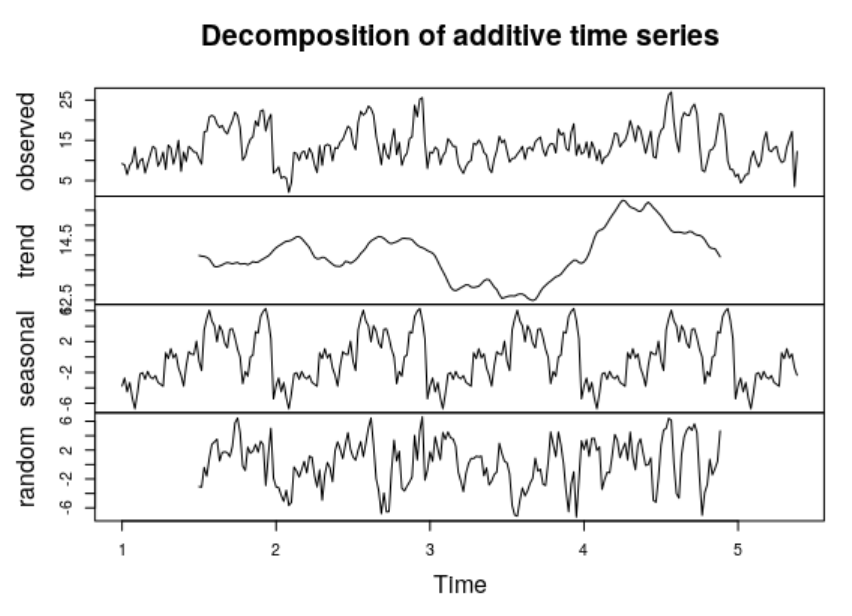
\includegraphics[scale=0.31]{decomp-diario.png}  %el parámetro scale permite agrandar o achicar la imagen. En el nombre de archivo puede especificar directorios
	\caption{Descomposición clásica de la serie temporal diaria} 
	\label{fig:decomp-diaria}
\end{figure}

Estudiando la tendencia, vemos que no tiene parecido a ninguna función conocida para realizar una aproximación funcional. Además, la variación es apenas de 2ºC, por lo que asumimos que la serie no tiene tendencia, por lo que forma parte del ruido. Respecto a la estacionalidad, fijo el periodo en 60, puesto que más o menos es el número de días que pasan desde un día hasta el mismo día en otro año (según la serie temporal generada solamente con los días de febrero y marzo de cada año). Por tanto, repito ese patrón de estacionalidad durante los distintos periodos y se lo resto a la serie, quedando así:

\begin{figure}[H] %con el [H] le obligamos a situar aquí la figura
	\centering
	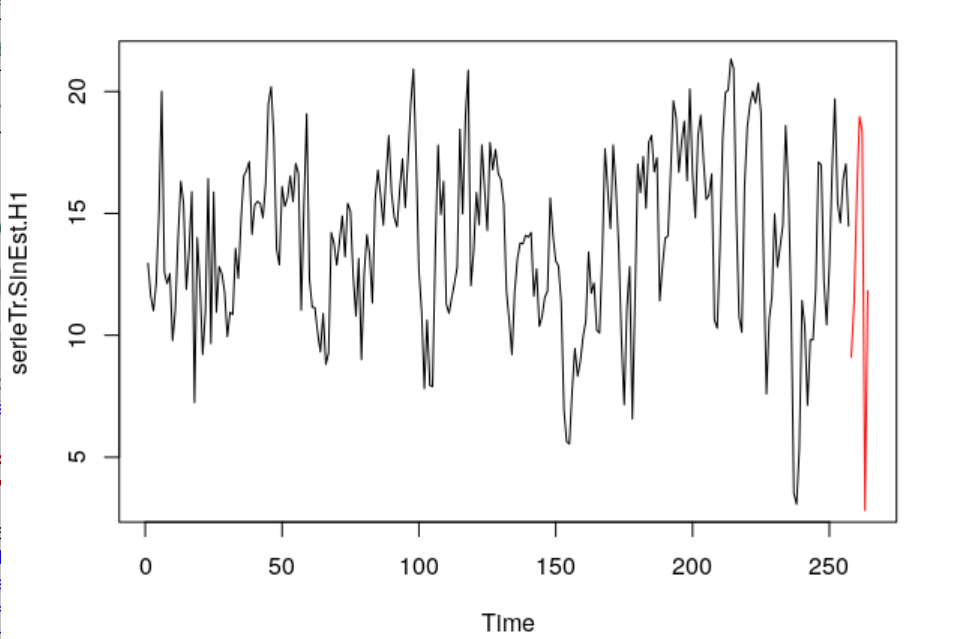
\includegraphics[scale=0.25]{diaria-Sin-Est.png}  %el parámetro scale permite agrandar o achicar la imagen. En el nombre de archivo puede especificar directorios
	\caption{Serie sin estacionalidad (en rojo el conjunto de test)} 
	\label{fig:diaria-sinest}
\end{figure}

Si nos centramos en la serie de la estación mensual

\begin{figure}[H] %con el [H] le obligamos a situar aquí la figura
	\centering
	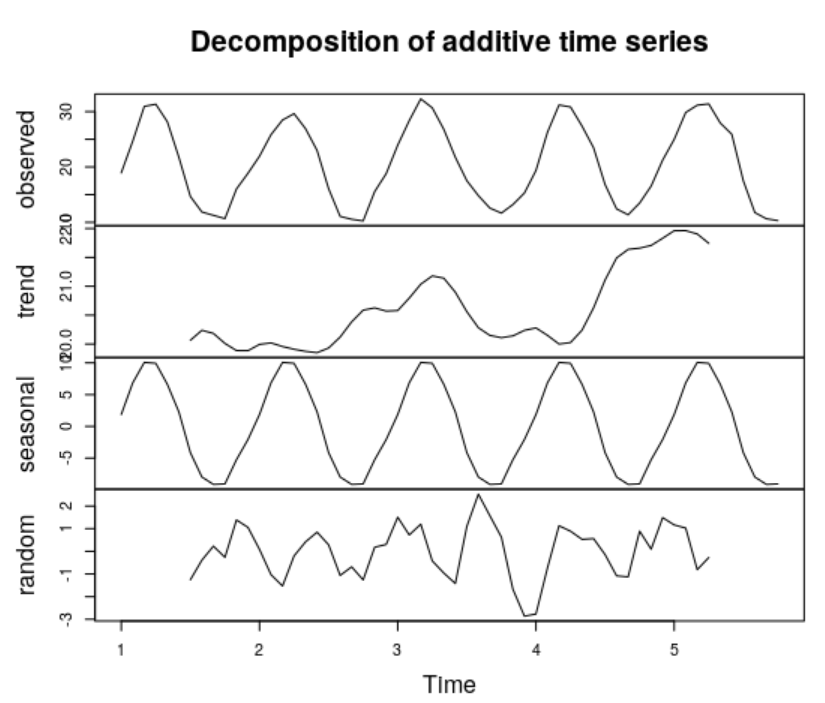
\includegraphics[scale=0.31]{decom-mensual.png}  %el parámetro scale permite agrandar o achicar la imagen. En el nombre de archivo puede especificar directorios
	\caption{Descomposición clásica de la serie temporal mensual} 
	\label{fig:decom-mensual}
\end{figure}

Volvemos a encontrarnos un patrón similar en la tendencia, que vuelvo a asemejarla a ruido, y una estacionalidad muy clara que elimino con la misma metodología que en el caso diario, obteniendo

\begin{figure}[H] %con el [H] le obligamos a situar aquí la figura
	\centering
	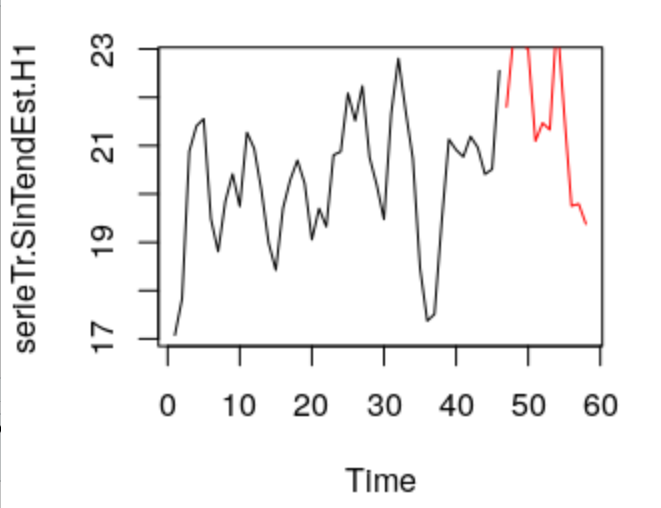
\includegraphics[scale=0.31]{trtsNE-mensual.png}  %el parámetro scale permite agrandar o achicar la imagen. En el nombre de archivo puede especificar directorios
	\caption{Serie sin estacionalidad (en rojo el conjunto de test)} 
	\label{fig:trtsNE-mensual}
\end{figure}

\subsection{Estacionariedad}

Una serie es estacionaria cuando sus propiedades no dependen del momento temporal en el que sea observada. Por tanto, una serie temporal con tendencia o estacionalidad no puede ser estacionaria, ya que la tendencia y la estacionalidad afectan al valor de la serie temporal en diferentes momentos (\cite{hyndman}) (por ese motivo pretendemos eliminar la estacionalidad y la tendencia en el apartado anterior). La estacionariedad se comprueba a través del test de Dickey-Fuller (\cite{df}), que mide si $\Phi = 0$ en
$$y_t = \alpha + \beta t + \Phi y_{t-1} +e_t$$
que se escribe como
$$\Delta y_t = y_t - y_{t-1} = \alpha + \beta t + \gamma y_{t-1} +e_t$$

siendo $y_t$ los datos de la serie. El test de Dickey-Fuller Aumentado permite procesos autoregresivos de orden superior incluyendo $\Delta y_{t-p}$ en el modelo. La hipótesis nula para ambos tests es que los datos son no estacionarios, por lo que se pretende obtener un p-valor menor que 0.05 para rechazarla. 

En el que caso de que no tengamos una serie estacionaria (no podemos rechazar la hipótesis nula, el gráfico ACF no tiende rápidamente a cero sino lentamente...) se puede emplear un método para hacerla estacionaria: la diferenciación. Ciertas transformaciones, como el logaritmo, ayudan a estabilizar la varianza en las series temporales. La diferenciación, por su parte, ayuda a estabilizar la media de la serie eliminando cambios, por lo que reduce tendencias o estacionalidades residuales. En el caso que nos ocupa, utilizo la diferenciación para suavizar la serie temporal y obtener unas gráficas ACF y PACF más claras para los modelos posteriores, a pesar de que en la estación diaria, antes de diferenciar, el test de Dickey-Fuller ya indica que la serie es estacionaria. 

\subsection{Modelado de series temporales}

\subsubsection{Modelos autoregresivos}

En un modelo de regresión multiple, predecimos la variable usando una combinación lineal de los predictores. En un modelo autoregresivo, predecimos la variable de interés usando una combinación lineal de los valores pasados de la variable (de ahí autoregresivo) (\cite{hyndman}). Por tanto, un modelo autoregresivo de orden $p$ se puede escribir como

$$y_t = c + \Phi_1 y_{t-1}+ \Phi_2 y_{t-2}+\dots+\Phi_p y_{t-p}+ \epsilon_t$$,

donde $\epsilon_t$ es ruido blanco. Nos referiremos a este tipo de modelos como $AR(p)$. Generalmente, restringimos los modelos autoregresivos a datos estacionarios, en cuyo caso se requieren ciertas condiciones sobre los parámetros:
\begin{itemize}
	\item $AR(1): -1 < \Phi_1 <1$.
	\item $AR(2): -1 < \Phi_2 <1, \Phi_1 +\Phi_2 < 1, \Phi_2-\Phi_1<1$
\end{itemize}

Para $p\geq 3$, las restricciones son mucho más severas (\cite{hyndman}).

\subsubsection{Modelos de medias móviles}

En lugar de utilizar los valores anteriores para predecir la variable deseada, un modelo de medias móviles utiliza los errores de predicción anteriores en un modelo de regresión:

$$y_t = c + \epsilon_t + \theta_1 \epsilon_{t-1} + \theta_2 \epsilon_{t-2} + \dots + \theta_q \epsilon_{t-q}$$

Téngase en cuenta que cada valor $y_t$ puede interpretarse como una media móvil ponderada de algunos errores de predicción anteriores.

\subsubsection{Modelos ARIMA en R}

Elegimos los parámetros del modelo ARIMA (AR o MA) estudiando las gráficas ACF y PACF. En el caso de un modelo AR, para elegir el parámetro, utilizamos el último valor distinto de 0 (que se sale de los márgenes y resulta representativo, siendo los otros ruido). En el caso del modelo MA, examinamos la gráfica ACF en busca del último valor más representativo. \\

Una vez entrenados los modelos, es necesario comprobar la bondad del ajuste, es decir, hay que evaluar la aleatoriedad de los residuos (Test de Box-Pierce) para comprobar si el modelo tiene sesgo; la normalidad de los residuos (Test de Jarque Bera y Shapiro-Wilk). Si no se comprueban las hipótesis mencionadas, los modelos no tienen un comportamiento correcto y no serán buenos predictores, por lo que deberían ser descartados. Además, para dos modelos que cumplan las hipótesis estadísticas, es necesario utilizar algún criterio para decidir cuál tiene mejor rendimiento. Para ello, utilizamos el error cuadrático medio sobre las instancias de test y el criterio de información de Akaike, que se basa en

$$ AIC = 2k + n\log(\frac{RSS}{n})$$
siendo $k$ el número de grados de libertad, $n$ el número de datos y $RSS$ la suma de los cuadrados de los residuos. 
\newpage
\section{PARTE PRÁCTICA}

\subsection{Estación diaria}

\subsection{Estación mensual}

\newpage
\section{Bibliografía}

%------------------------------------------------

\bibliography{citas} %archivo citas.bib que contiene las entradas 
\bibliographystyle{plain} % hay varias formas de citar

\end{document}
